% !TEX root = ../These_TOC.tex
\chapter{Explorer visuellement des données de simulation massives pour analyser le comportement d'un modèle.}
\begin{center}
	{\large Version \hl{2018-08-27}}\\
	\hl{Corrections de la partie 5.1 à 5.2.3 non prises en compte.}

\end{center}
\minitoc

\clearpage

% Plan initial
%\section{Explorati&on manuelle}
%
%\subsection{Paramètres}
%
%\subsection{Indicateurs}
%
%\subsection{Plans d'experience}
%
%\section{Exploration Systématique}
%
%\section{Scénarios}
%
% Plan détaillé pour demande dérogation 6ème année (2018-05)
%\section{Comprendre un modèle en l'utilisant}
%\subsection{Explorer un modèle en multipliant les simulations}
%\subsection{Explorer le comportement d'un modèle en multipliant les experimentations}
%\subsection{Explorer en comparant}
%
%\section{Exploration visuelle guidée d'un modèle : analyse de SimFeodal}
%\subsection{Comprendre les variations des paramètres de SimFeodal}
%\subsection{Définir des plans d'experience pour explorer SimFeodal}
%\subsection{Explorer la variabilité de l'aléa d'un modèle fortement stochastique}
%
%\section{Comprendre un modèle par son exploration systématique}
%\subsection{Compréhension et validation des modèles théoriques}
%\subsection{\textit{Curse of dimensionality} : comment systématiser l'exploration d'un modèle descriptif complexe}
%\subsection{Plan complet vs exploration des possibles}
%
% Plan du 2018-06-12
%

\section{Capter les sorties de SimFeodal}
\label{sec:sorties-simfeodal}
Pour évaluer un modèle, on s’appuie sur plusieurs indicateurs de sortie de simulation, de types divers (indicateurs numériques, graphiques, cartographiques etc., \hl{cf. chapitre 3, partie théorique}).
Quand le nombre d'indicateurs devient important, comme c'est le cas dans le modèle SimFeodal (chap 3, partie présentation des indicateurs), la consultation des indicateurs pendant le déroulement d'une simulation devient difficile.
La complexité de ces indicateurs augmente, elle-même, dans le cas d'un modèle stochastique comme SimFeodal, où il est nécessaire de multiplier les réplications afin d'avoir une idée fiable de la tendance du modèle.
Le travail de paramétrage d'un modèle requiert de plus de mener différentes expériences, c'est-à-dire de faire varier les paramètres (chap 4) d'un modèle, démultipliant encore la masse des sorties, et avec elle, la complexité nécessaire à leur étude.
Nous détaillons ici les contraintes qu’entraînent ces différentes spécificités des données issues de simulation de SimFeodal.

	\subsection{Masse des données}
	Dans un premier temps, il convient de noter que l'ensemble des indicateurs observés en sortie de SimFeodal reposent sur des données qu'il est nécessaire de produire et d'enregistrer tout au long de la simulation.
	Ainsi, pour pouvoir tracer une courbe de l'évolution du nombre d'agrégats au cours du temps, encore faut-il avoir accès à cette information, et dès lors, enregistrer, à chaque pas de temps, cette valeur dans un fichier numérique adapté.
	Cette information, en tant que telle, est assez faible, aussi bien en valeur sémantique qu'en valeur prise en mémoire.
	Pour autant, on a montré que les indicateurs de sortie étaient nombreux, et avec eux, la quantité de valeurs à stocker augmente.
	Ainsi, à chaque pas de temps, il faudra enregistrer les valeurs de plusieurs variables.
	Ce comportement est habituel, et un format de données tabulaire se prête bien à un tel enregistrement : une ligne pour chaque pas de temps, et une colonne pour chaque variable à enregistrer.
	On obtiendrait ainsi en sortie de simulation un tableau contenant 18 lignes (le nombre de pas de temps de SimFeodal) et une cinquantaine de colonnes, ce qui serait assez raisonnable.

	Il faut toutefois considérer un aspect important de l'exploration de données issues de simulations : la production de ces données a un coût temporel important, c'est-à-dire que l’exécution d'une simulation requiert un certain temps (3 à 4 minutes pour une exécution du modèle SimFeodal dans la version présentée dans le \hl{chapitre 2}).
	Si l'on considère de plus que les indicateurs peuvent évoluer au cours des étapes de construction et de paramétrage d'un modèle (cf. \hl{encadré chap 3}), on a alors tout intérêt à prévoir ce cas, et donc à enregistrer l'état de variables qui ne seraient pas encore mobilisées pour la production d'indicateurs.
	Dans le cas contraire, pour chaque changement ou ajout d'indicateur, il faudrait relancer des exécutions du modèle sur l'ensemble des jeux de paramètres précédents afin d'être en mesure d'avoir des indicateurs comparables entre les versions.

	Enregistrer l'ensemble des variables d'un modèle est aisé dans le cas d'un modèle théorique simple, par exemple dans le cas d'un modèle comme celui de Schelling (\hl{ref}). Cela se complique quand il s'agit d'enregistrer les variables d'un modèle plus complexe comme SimFeodal.
	Celui-ci comprend ainsi bien plus de variables globales, représentant l'état du système dans son ensemble à chaque instant.
	Surtout, SimFeodal est un modèle qui voit interagir plusieurs types d'agents, chacun situés à différents niveaux de granularité spatiale et sociale.
	Afin d'avoir tous les éléments en main une fois la simulation achevée, il est donc nécessaire d'enregistrer l'ensemble des variables non seulement globales, mais aussi afférentes à chacun des types d'agents.
	D'un tableau de données exhaustif en sortie du modèle de Schelling, on passe donc à plusieurs tableaux, dont les variables respectives seront propres à chaque type d'agent.

	A ce niveau, l'information en sortie est encore relativement contenue : il y a cinq types d'agents, ayant chacun une douzaine d'attributs, dans SimFeodal. On pourrait donc se contenter de ces cinq tableaux contenant 18 lignes (les pas de temps) et la douzaine d'attributs propres, comme c'est classiquement le cas dans (\hl{trouver exemple}).

	Reste encore un obstacle majeur à un enregistrement suffisant du déroulement d'une simulation : une part importante des indicateurs s'appuie sur des données individuelles et non agrégées.
	Ainsi, enregistrer une situation globale des paroisses à chaque pas de temps permet par exemple d'en examiner le nombre, la superficie moyenne ou encore le nombre moyen de paroissiens desservis.
	Mais cela ne permet en aucun cas d'en dresser une cartographie, ce qui nécessite, par définition, d'enregistrer la géométrie de chaque paroisse à chaque pas de temps.
	De même, on a vu que les indicateurs pouvaient être amenés à évoluer : si l'on enregistre un nombre de paroissiens moyen à chaque pas de temps, puis que l'on décide après coup de comparer non plus cette moyenne, mais une médiane, ou encore d'observer la forme de cette distribution, on se trouve alors dans une situation impossible requérant de ré-exécuter les simulations après avoir adapté l'indicateur voulu.

	Pour se prémunir de cette situation, on a donc fait le choix, dans SimFeodal, d'enregistrer les états des variables à des niveaux d'agrégation multiples, y compris au niveau de l'agent individuel. Dans le cas des paroisses, le volume de données résultant reste contenu : on obtient un tableau d'environ 2000 lignes\footnote{
	Avec une moyenne de 120 paroisses, cela représente $18_{\text{\tiny ~[pas de temps]}} \times 120_{\text{\tiny ~[paroisses]}} \approx 2000$ lignes pour chaque simulation.
	} et une dizaine de colonnes\footnote{
	Les identifiants de la simulation (nom, graine aléatoire), le pas de temps, l'identifiant de la paroisse, puis les différents attributs et la géométrie.
	}.
	L'enregistrement systématique de chaque agent est toutefois bien plus gênant dans le cas d'autres agents, par exemple les foyers paysans. Pour ceux-là, et parce qu'on doit être en mesure d'étudier les liens entre satisfactions et choix de déplacements, ou encore d'observer la composition précise de la distribution des satisfactions, il est aussi nécessaire d'enregistrer les attributs de chacun. Avec $4000$ foyers paysans à chaque tour, les données changent ainsi d'ordre de grandeur\footnote{
	$18_{\text{\tiny ~[pas de temps]}} \times 4000_{\text{\tiny ~[foyers paysans]}} \approx 70~000$ lignes pour une exécution du modèle.
	} : chaque simulation requiert de générer un fichier contenant des dizaines de milliers de lignes, pour un total, pour cet unique fichier, d'une dizaine de mégaoctets occupés.

	A terme, pour enregistrer un état représentatif d'une simulation, c'est-à-dire avoir suffisamment d'éléments numériques pour pouvoir générer les indicateurs de sortie et prévoir une partie de leur évolution, la masse de données produite est assez conséquente.

	\subsection{Réplications}

	Comme on l'a vu dans le \hl{chapitre 3}, une simulation ne suffit toutefois pas à évaluer le modèle.
	SimFeodal est ainsi un modèle stochastique, c'est-à-dire qu'une large partie des mécanismes qui l'animent sont basés sur des tirages aléatoires.
	Cet aléa est évident dans les mécanismes faisant appel à un tirage, par exemple le choix de déplacement ou non d'un foyer paysan (\hl{cf. chap2, mécanisme déplacement}).
	Dans le cas de ce mécanisme, un foyer paysan mobile se déplacera selon une probabilité dépendant de sa satisfaction.
	Et s'il y a probabilité, il y a donc aléa.
	Même avec une forte satisfaction --- $0.99$ par exemple ---, il reste donc $1\%$ de chance qu'un foyer se déplace, ce qui, sur un grand nombre de tirages (chaque foyers paysans, à chaque pas de temps), a une forte probabilité de réalisation.
	L'aléa a donc un poids important dans ce type de mécanisme.

	Pour autant, même dans des mécanismes plus anodins, l'aléa est fortement présent, étant au cœur de la conception de SimFeodal.
	Ainsi, le simple ordre d’exécution du mécanisme de déplacement des foyers paysans peut avoir une importance considérable.
	\hl{Cet exemple est faux, en trouver un juste où l'ordre d’exécution importe dans SimFeodal et le développer.}

	On pourrait objecter qu'en considérant les agents de manière agrégée, donc globale, les probabilités s'effectuent sur suffisamment d'individus pour présenter un résultat cohérent et déterministe au niveau de la population dans son ensemble.
	En corollaire, le comportement de chaque agent serait régulé par tant de variables aléatoires qu'on entrerait dans le cadre d'application de la loi forte des grands nombres, les agents adoptant alors en moyenne un comportement proche de l’espérance (moyenne théorique) de chaque tirage.
	Avec ces considérations, on pourrait justifier le déterminisme probable des différentes exécutions de SimFeodal.

	SimFeodal n'est toutefois pas simplement un modèle stochastique, mais avant tout, un modèle complexe, c'est-à-dire s'inscrivant dans le champs des systèmes complexes. Sans vouloir ici entrer dans les détails des implications et raisons de ceci, on peut simplement en retenir, qu'un modèle tel que SimFeodal est extrêmement sensible aussi bien aux conditions initiales qu'aux différents tirages aléatoires.
	\hl{A développer sérieusement ici, ou bien dans les chapitres 1 ou 2. Il faudra de toute façon faire un point quelque part sur les systèmes complexes, l'émergence etc.}
	Pour illustrer, on peut s'appuyer sur un exemple ---
	fictif jusqu'ici dans les différentes exécutions du modèle
	--- possible : à l'initialisation, tous les foyers paysans, placés aléatoirement dans l'espace, seraient ici concentrés dans un espace faible.
	Seul un énorme agrégat émergerait donc, et aucun pôle ne serait susceptible dès lors de diviser cet agrégat géant.
	On atteindrait ainsi une situation très éloignée de l'empirie, et très éloignée aussi des réalisations habituelles du modèle.
	En présence d'un seul agrégat, les possibilités de développement d'attracteurs (châteaux et paroisses) pourraient alors tout aussi bien être fortes que faibles.
	À partir de cette configuration initiale, on ne peut savoir si la situation convergerait vers un agrégat \og paradisiaque\fg{}, extrêmement développé et doté de pôles satisfaisants, ou au contraire, vers un agrégat \og prison \fg{}, où aucun des foyers paysans ne serait satisfait, mais n'aurait non plus d'alternative.

	Cet exemple fictif, volontairement caricatural, ne s'est jamais produit jusqu'ici, mais le cas échéant, encore faudrait-il pouvoir le repérer, pour éventuellement l'isoler d'autres simulations.
	On ne peut donc pas raisonner sur une unique simulation pour évaluer un jeu de paramètres (\hl{cf. chap 3}), mais on ne peut pas non plus se contenter de récupérer des différentes réplications et d'en tirer une moyenne (selon qu'on s'intéresse par exemple à la tendance générale) ou un écart-type (si l'on cherche justement à observer les variations que peut entraîner l'aléa).

	Pour ces raisons, et pour être en mesure d'embrasser l'entière diversité des sorties de simulations issues de variation de la graine aléatoire, il est donc nécessaire de mener plusieurs réplications de chaque simulation, et d'enregistrer l'entièreté des sorties de simulations dans chacun des cas.
	Le jeu de données produit par une simulation, contenant quelques dizaines de milliers de lignes, est ainsi obligatoirement multiplié par le nombre de réplications.
	Pour l'exploration de SimFeodal, après différents tests, ce nombre a été fixé à $20$ réplications (\hl{J'en aurais sans doute parlé dans le chapitre 3 (évaluation), mais à laisser ici jusqu'à ce que ce soit certain.}).
	La dizaine de mégaoctet issue d'une simulation devient donc approximativement 200 mégaoctets, et le nombre de lignes contenues, par exemple pour les foyers paysans, passe d'à peu près $70~000$ à $1~400~000$\footnote{
	Si cette quantité de données semble tout à fait raisonnable et peut largement être traitée sur un ordinateur classique, on peut toutefois noter qu'elle dépasse toutefois déjà le maximum de lignes ($2^{20}, \approx 1~000~000$) que les tableurs classiques ---
	LibreOffice ou Microsoft Excel dans leurs dernières versions en 2018
	--- sont en capacité de gérer.
	}.

	\subsection{Expériences}

	Comme décrit dans le \hl{chapitre 4}, le paramétrage de SimFeodal a demandé plusieurs étapes.
	Chacune de ces étapes représente, qui plus est, plusieurs sous-étapes, faites d'essais et d'erreurs, en faisant varier à chaque fois les valeurs de paramètres de SimFeodal.
	Afin de construire le modèle, puis de l'explorer de manière plus systématique, il a donc été nécessaire de tester des dizaines de configurations de paramètres.
	L'objectif étant de comparer, à chaque fois, les résultats en sortie de simulation d'un nouveau jeu de paramètres testé, il était indispensable de conserver, au minimum, l'ensemble des jeux de données de la version précédemment testée du modèle.
	
	Cela n'est pourtant pas suffisant, pour plusieurs raisons aussi bien éthiques que méthodologiques.
	En premier lieu, pour des impératifs de reproductibilité (\hl{Ça aussi faudrait quand même en parler quelque part. Chap. 7 ?}) de la démarche engagée, aussi bien que pour la simple capacité à restituer honnêtement et rigoureusement les étapes suivies, il était nécessaire de conserver l'ensemble des indicateurs de sortie de simulations correspondant à chaque étape ou sous-étape.
	Cette démarche de paramétrage s'inscrivant ainsi sur une durée assez étalée, et suivant surtout un avancement non linéaire fait d'allers-retours, il était indispensable de documenter autant que possible chaque avancée, et pour cela, de conserver l'ensemble des résultats en résultant.

	Une autre contrainte, méthodologique, déjà évoquée (\hl{cf. encadré incrémentalité des indicateurs dans chap. 3}), complexifie toutefois encore la tâche.
	Ainsi, les indicateurs jugés utiles évoluent tout au long des étapes de paramétrage.
	Or, pour pouvoir comparer les résultats de simulations issues de jeux de paramètres différents, encore faut-il disposer d'indicateurs comparables, et donc, identiques dans leur définition.
	Si l'on ne conserve que les indicateurs de chaque simulation, on ne peut donc les ajuster sans avoir accès aux données sources ayant permis de les produire.

	Pour ces raisons, il n'était pas possible de mener un travail de paramétrage de SimFeodal sans conserver l'ensemble des données produites, c'est-à-dire l'ensemble des attributs de l'ensemble des agents de chacune des réplications, tout cela pour chacune des expérimentations.

	En supposant que les 8 étapes présentées dans le chapitre précédent (\hl{ref chap2, étapes}) soient ne serait-ce que constituées de 3 sous-étapes chacune --- ce qui est bien en deçà de la réalité ---, on obtient donc 24 jeux de paramètres à stocker, puis à devoir mobiliser.
	Cela représente alors une somme considérable de données, qui se chiffrent en dizaines de millions d'enregistrement\footnote{
	$18_{\text{\tiny ~[pas de temps]}} \times 4000_{\text{\tiny ~[foyers paysans]}} \times 20_{\text{\tiny ~[réplications]}} \times 24_{\text{\tiny ~[jeux de paramètres]}} \approx 35~000~000$ de lignes enregistrées pour les seuls foyers paysans.
	}.
	Si cela ne représente jamais que quelques gigaoctets de données, ce que quiconque a désormais l'habitude de manipuler dans un cadre personnel, en terme de traitement, cette masse de données est à la limite de ce que l'on peut traiter sur un ordinateur individuel.
	Ainsi, selon une approximation courante, on ne peut charger en mémoire de données d'une taille supérieure à la moitié de la mémoire vive disponible, sans même prendre en compte les autres éventuels processus en cours.
	Avec 5 Go de données , il faut donc disposer d'un ordinateur personnel possédant au moins une douzaine de gigaoctets de mémoire vive, et encore, au prix d'un traitement extrêmement lent et bloquant.
	
	Et encore, on ne mentionne ici que les expérimentations issues des étapes de paramétrage.
	Les phases suivantes d'exploration du comportement du modèle, par exemple autour de variations systématiques de valeurs de paramètres en vue de calibration, demandent ainsi d'exécuter, et donc d'enregistrer, une masse bien plus importante de simulations.

	\subsection{Des données aux indicateurs}\label{subsec:donnees-indicateurs}
	Dans l'ensemble, l'enregistrement et la sauvegarde des données issues de simulations, en vue de leur mobil0isation pour produire les indicateurs de sortie, se révèle une contrainte importante dans la compréhension du comportement d'un modèle.
	C'est particulièrement le cas pour SimFeodal, où l'on ne peut se contenter de produire à la volée les indicateurs, pour des raisons de reproductibilité théorique et pratique.
	
	La masse de données en sortie est impressionnante et requiert donc premièrement d'utiliser des outils adaptés à la manipulation de grands jeux de données.
	Cela exclue de fait l'outillage traditionnel de la géographie quantitative, ne laissant par exemple pas la possibilité d'utiliser les outils à interface graphique classiques.
	Au contraire, face à des données de cet ordre, seules des solutions statistiques, basées sur des analyses en ligne de commande, peuvent être mobilisées.
	Ces solutions doivent en plus être appuyées par des capacités de calculs importantes, sans toutefois justifier encore l'usage de technologies de calcul intensif.
	Cela pose une première contrainte dans l'universalité de l'analyse, en particulier dans un contexte interdisciplinaire porteur d'une large hétérogénéité en matière de pratiques quantitatives : il n'est pas possible de juste envoyer les jeux de données produits aux thématiciens, qui ne pourraient en l'état pas en tirer les indicateurs nécessaires.

	Dans un second temps, et c'est là la contrainte principale, cette masse de données doit servir à la production d'indicateurs, nombreux et divers aussi bien dans leur forme que dans les caractéristiques des processus qu'ils décrivent (\hl{ref. chap. 3, indicateurs}).
	Les mêmes raisonnement que pour les données s'appliquent ainsi aux indicateurs.
	Si on peut prendre en compte la variabilité des réplications directement dans les indicateurs produits (par exemple avec des représentations graphiques de type \textit{box-plot} qu'adoptent une forte partie des indicateurs), ce n'est ni possible ni souhaitable entre les différentes expériences.
	De fait, chaque expérience doit pouvoir être comparée aux précédentes sur la base de leurs seules réplications respectives.
	Dès lors, la raison d'être des indicateurs de sortie est de rendre possible une comparaison, indicateur par indicateur, entre chacune des expériences. 
	Il est donc indispensable de générer, pour chaque expérience, l'ensemble des indicateurs. En ne considérant ici encore que 24 expériences, cela fait donc déjà plusieurs centaines\footnote{
	En considérant ainsi une trentaine d'indicateurs, on obtient donc $30{\text{\tiny ~[indicateurs]}} \times 24_{\text{\tiny ~[jeux de paramètres]}} \approx 700$ indicateurs uniques.
	} d'indicateurs (\cref{tbl:hierarchie-simulations}).

	\begin{table}[!]
		\raggedleft
		\resizebox{.85\textwidth}{!}{%
			\begin{tabular}{N|M{2.5cm}|M{2.5cm}|M{2cm}|M{3.5cm}|M{4.5cm}|N|}
				\hline
				&	& \multicolumn{2}{|c|}{\thead{Données}} & \multicolumn{2}{|c|}{\thead{Indicateurs}} \\ \hline
				& \thead{Intitulé} & \thead{Quantité} & \thead{Poids} & \thead{Type} & \thead{Quantité} & \\[25pt] \hline
				\tikzmark{a}& Une simulation & \makecell{$\approx 10^5$ lignes}& $\approx 10$ Mo & \begin{tabular}[c]{@{}l@{}}Visualisations\\ en direct\end{tabular} & \makecell{$\approx 10$ indicateurs}  & \\[50pt] \hline
				\tikzmark{b}& Une expérience & \makecell{$\approx 10^6$ lignes} & $\approx 200$ Mo & Indicateurs de sortie & \makecell{$\approx 30$ indicateurs\\(variabilité des\\réplications)} & \\[50pt] \hline
				\tikzmark{c} & \makecell{Huit étapes\\de\\paramétrage} & \makecell{$\approx ~10^7$ lignes} & $\approx 5$ Go & Indicateurs de sortie & \makecell{$\approx 700$ indicateurs\\ (à comparer entre\\les expériences)} & \\[50pt] \hline
			\end{tabular}%
			\tikz[overlay,remember picture] \draw[->, >=latex', bend right=90, thick, dashed] (a.west) to node[pos=.5, left, align=center, xshift=0pt]{$\times 20$\\$\textrm{réplications}$} (b.west) ;
			\tikz[overlay,remember picture] \draw[->, >=latex', bend right=90, thick, dashed] (b.west) to node[pos=.5, left, align=center, xshift=0pt]{$\times \approx 24$\\$\textrm{expériences}$} (c.west) ;
		}
		\caption{Synthèse de la multiplication des données et indicateurs selon la hiérarchie des simulations.}
		\label{tbl:hierarchie-simulations}
	\end{table}

	Le choix ayant été fait de mener une comparaison visuelle (\hl{ref. dans chapitre 3 : indicateurs uniques vs fonctions objectifs}), on imagine dès lors que celle-ci va être difficile en présence de tant d'indicateurs.

	En sus de la contrainte de l'enregistrement et de la production des indicateurs, le verrou majeur à la compréhension des phénomènes modélisés dans SimFeodal est donc la simple capacité à visualiser et à explorer l'ensemble des indicateurs de sortie.
	Ce qui doit de plus être rendu accessible y compris pour un auditoire non habitué à la manipulation de nombreuses données et sorties quantitatives.
	
\clearpage
\section{Comment explorer les données de SimFeodal ?}

	Pour évaluer une expérience de SimFeodal, on doit passer en revue une trentaine d'indicateurs de sortie de simulation.
	Cette évaluation ne vise pas à aboutir à une note unique, mais plutôt à une idée de la capacité de l'expérimentation à reproduire les dynamiques modélisées.
	Il ne s'agit donc pas a proprement parler d'une évaluation du modèle, mais plutôt d'une exploration de son comportement en fonction des mécanismes et valeurs de paramètres choisis.
	Pour mener cette exploration, il convient d'utiliser des outils adaptés, c'est-à-dire de disposer de solutions techniques permettant le calcul et l'affichage des indicateurs à partir des données produites par le modèle.
	Dans le travail mené autour de SimFeodal, plusieurs solutions ont été utilisées au cours des différentes étapes de construction du modèle.
	La restitution purement chronologique de ces solutions ne revêt pas d'intérêt propre, mais les contraintes accumulées au cours de la construction du modèle et les choix devant permettre de les dépasser nous paraissent très largement génériques.
	Nous justifions donc ici la succession de choix d'outils d'explorations au prisme des verrous dans l'exploration que chacun a permis de débloquer, ce qui dresse par là-même un portrait des solutions méthodologies d'exploration de données de simulations dont on peut faire usage selon les contraintes générales des modèles.\hl{Pas clair, à reprendre, mais l'idée est là.}
	
	\subsection{Observation en direct vs a posteriori}\label{subsec:observation-a-posteriori}

	Classiquement, le premier réflexe d'un modélisateur, du moins pour les modèles à base d'agents, est de définir des sorties graphiques pour accompagner son modèle.
	Les différentes plate-formes de modélisation agent mettent d'ailleurs régulièrement en avant les possibilités de représentations qu'offrent leurs environnements (\hl{ref blogs Gama, NetLogo 3D, GeoMASON, Repast}).
	Visualiser le déroulement d'un modèle ``en direct'' (\textit{online} dans Grignard \& Drogoul2017) offre ainsi de nombreux avantages (\hl{cf. HDR Arnaud, en sortir une citation et/ou un listing}).

	Dans l'exploration de SimFeodal, la création en direct de quelques graphiques correspondant à des indicateurs étudiés permet de vérifier, avant le lancement d'une série de simulations, que le déroulement de la simulation ne présente pas de forte incohérence et qu'un \textit{bug} n'a pas été introduit involontairement.
	Pourtant, deux contraintes limitent fortement le recours à ce type de visualisation en direct des simulations.

	La première contrainte, déjà évoquée plus haut, est que le modèle SimFeodal est fortement stochastique.
	Dès lors, la visualisation des indicateurs d'une simulation particulière ne suffit pas à estimer le comportement du modèle.
	C'est bien pour cela que les indicateurs choisis pour l'évaluation de SimFeodal prennent presque tous en compte la variabilité des résultats induite par l'exécution de réplications.

	Certains environnements techniques (\hl{ref à multi-simulation dans Gama}) permettent toutefois de mener concomitamment plusieurs réplications d'un même modèle et de visualiser directement pendant l'exécution les résultats des réplications agrégés.
	La première contrainte, liée à la nécessaire étude des réplications du modèle, peut donc être dépassée en adaptant l'implémentation du modèle pour faire usage de ces capacités de multi-simulation.

	La seconde contrainte est plus cruciale dans le cas de SimFeodal et invalide l'usage des méthodes de visualisation en direct.
	On l'a vu, l'exploration des sorties de simulation du modèle repose sur la consultation d'une trentaine d'indicateurs, parfois très spécifiques au cas d'étude de SimFeodal.
	Outre le fait qu'il serait concrètement difficile de représenter tous ces indicateurs au sein de l'interface graphique d'une plate-forme de simulation agent, la temporalité de l'exécution d'une simulation (ou même des réplications nécessaires) est bien plus courte que celle requise pour la compréhension des résultats produits.
	Les indicateurs de sortie de simulation demandent ainsi un examen approfondi avant d'être en mesure de juger de leur adéquation aux attentes thématiques.
	Cet examen ne peut que difficilement être réalisé en direct, qui plus est quand il demande de faire appel, dans le cadre de co-construction inhérent à SimFeodal, à plusieurs points de vue.
	Les modalités mêmes de l'exploration des sorties de SimFeodal requièrent donc que les indicateurs soient visibles et explorables à des temporalités différentes, par des chercheurs différents, depuis des lieux différents.
	Pour un même chercheur, l'évaluation n'étant pas une étape unique et finie, il est utile de pouvoir revenir sur les résultats à différents moments, ne serait-ce que pour comparer les nouveaux résultats produits à ceux générés par des expérimentations précédentes.

	Il est donc indispensable que les indicateurs soient enregistrés et consultables simplement à tout moment, ce qui élimine de fait la visualisation des indicateurs en direct pendant l'exécution des simulations comme unique méthode d'exploration du comportement de SimFeodal.

	La visualisation en direct n'est donc pas mobilisable en tant que telle, mais elle peut tout de même, comme dans un usage très classique, être utilisée comme un outil de validation interne pour tester chaque modification dans les valeurs de paramètres.
	Visualiser une seule simulation, avant d'en exécuter les réplications nécessaires, permet ainsi déjà de vérifier que les modifications apportées dans les valeurs de paramètre ou dans les mécanismes n'ont pas entraîné l'apparition de \textit{bugs} ou d'incohérences immédiatement visibles.

	Nous avons donc choisi de doter SimFeodal d'une interface graphique, très sommaire, mais permettant des allers-retours rapides entre l'implémentation et l'exécution.
	Cette interface n'affiche qu'un nombre réduit d'indicateurs (\autoref{fig:simfeodal_gui_indicateurs}), ainsi qu'une représentation cartographique (\autoref{fig:simfeodal_gui_carte}) utile à une analyse rapide du comportement d'ensemble du modèle.

\begin{figure}[H]
	\captionsetup{width=\linewidth}
	\includegraphics[width=0.5\linewidth]{img/SimFeodal_GUI_FP.png}
	\includegraphics[width=0.5\linewidth]{img/SimFeodal_GUI_seigneurs.png}
	\caption{Visualisations intégrées à l'interface graphique de SimFeodal : indicateurs liés aux foyers paysans et aux seigneurs.} 
	\label{fig:simfeodal_gui_indicateurs} 
\end{figure}

\begin{figure}[H]
	\captionsetup{width=\linewidth}
	\includegraphics[width=\linewidth]{img/SimFeodal_GUI_carte.png}
	\caption{Visualisations intégrées à l'interface graphique de SimFeodal : cartographie synthétique de l'espace modélisé.} 
	\label{fig:simfeodal_gui_carte} 
\end{figure}
	
	Ces représentations ne suffisent pas et ne remettent aucunement en cause les constats de leur inadéquation aux contraintes d'ensemble de l'évaluation de SimFeodal.
	Elles complètent cependant la démarche d'évaluation du modèle par l'ajout d'une étape de contrôle préalable au lancement d'expériences,ce qui ne peut être qu'avantageux.

	\subsection{Générer les indicateurs}

	Si la production des indicateurs doit donc nécessairement être réalisée en aval de l'execution des simulations (\textit{offline} dans Grignard \& Drogoul 2017), encore faut-il disposer d'outils adaptés au traitement des données produites, c'est-à-dire répondant aux contraintes identifiées auparavant (\autoref{subsec:donnees-indicateurs}).
	La contrainte principale est d'être en mesure de gérer la masse de données produites.
	On l'a vu, cela élimine d'office les outils de type tableurs, ou encore les outils de manipulation graphique de données les plus courants.
	Pour les raisons évoquées dans le chapitre 1 (\hl{Positionnement : pourquoi utiliser des outils libres ?}), seules les solutions techniques non-propriétaires étaient envisageables.

	Certains outils graphiques, basés sur des logiciels libres en arrière-plan (PSPP, R Commander, Orange), sont extrêmement aisés à prendre en main et auraient pu constituer un bon choix.
	Pourtant, avec une trentaine d'indicateurs à produire pour chaque expérience, donc de manière régulière, nous avons préféré nous tourner vers des outils plus orientés vers une interface en ligne de commande (\textit{Command Line Interface}, abrégés \textit{CLI}).
	
	L'utilisation de CLI a plusieurs interêts gravitant autour de la reproductibilité des traitements.
	En premier lieu, ils permettent une adaptation aisée et rapide aux différents jeux de données.
	Ainsi, partant du principe que les données générées par les réplications et expérimentations sont de même structures, il suffit généralement de modifier le chemin d'entrée des fichiers résultants pour reproduire à l'identique une analyse sur un nouveau jeu de données.

	De manière plus technique et interne à la génération des indicateurs, on peut remarquer que les différents indicateurs de sortie de simulation choisis présentent souvent des caractéristiques communes, aussi bien dans le traitement nécessaire que dans les formats (graphiques) produits.

	Par exemple, la grande majorité des indicateurs reposent sur une première agrégation des données par réplication et pas de temps simulé, puis par une seconde agrégation montrant la variabilité des situations générées, au niveau de l'expérimentation donc.
	En terme de manipulation de données, seul l'indicateur statistique final, et éventuellement l'agent caractérisé, est ainsi modifié dans ces nombreux indicateurs de sortie.
	Le recours à des traitements en CLI permet ainsi un simple copier/coller, voir la création de fonctions dédiées, pour effectuer ces traitements très récurrents.

	Au niveau des sorties graphiques, et donc des indicateurs multi-dimensionnels (\hl{cf. chap 3 et schéma des indicateurs}), on peut aussi remarquer que la forme est assez largement identique : on représente les pas des temps (les années simulées) en abscisse, un indicateur statistique en ordonnée, et les figurés sont sous forme de \textit{box-plot} minimalistes (\og \textit{minimal boxplot}\fg{}, promus par Edward Tufte pour minimiser le ratio données-encre.\hl{Mettre les réfs de Tufte}).
	Là aussi, en disposant d'un environnement de type CLI, et qui plus est en faisant usage de solutions graphiques construites sur une syntaxe régulière et générique\footnote{
	On utilise pour tous ces graphiques le \textit{package} R \texttt{ggplot2}, qui repose sur la grammaire graphique conçue par Leland Wilkinson (\hl{ref}).
	}, il devient très confortable de n'avoir qu'a adapter un premier graphique conçu aux autres indicateurs souhaités.

	Avec ces solutions, il est facile de concevoir et d'implémenter les codes informatiques nécessaires à la génération des indicateurs de sortie de simulation.
	Cela est de plus, dans l'exécution de ces programmes, extrêmement rapides, les différents fichiers de sortie de simulation étant lus et parcourus un unique fois pour en tirer toutes les variables nécessaires à l'établissement des indicateurs.

	En sortie, on obtient une table synthétique (indicateurs numériques, \hl{cf. schéma chap. 3}) et de nombreux graphiques dans des formats vectoriels, donc aisément modifiables, par exemple pour publication, et surtout, lisibles et transférables très simplement.

	\subsection{Organiser les indicateurs en rapports paramétrables}

	Du point de vue de la manipulation, la création de fichiers informatiques indépendants correspondant aux différents indicateurs de sortie de simulation est extrêmement pratique : on peut facilement les échanger et les adapter, par exemple pour inclusion dans une publication.

	Du point de vue de la comparaison des résultats, cette forme n'est pourtant pas la plus adaptée.
	Si l'on peut facilement comparer un même indicateur portant sur deux expériences différentes, la tache se complique quand il s'agit d'avoir une vision globale des différences dans les indicateurs entre deux expériences.
	Pour cela, la démultiplication des fichiers correspondant aux indicateurs se révèle rapidement être un obstacle : on est alors amené à jongler entre de très nombreux fichiers.

	Pour rendre la comparaison des indicateurs plus aisée, en présence d'une forte diversité d'indicateurs, il convient donc, a minima, d'organiser les indicateurs.
	Nous entendons ici par organisation, une présentation structurée, suivant un certain ordre, identique selon les expériences, adapté à une évaluation des résultats du modèle SimFeodal.
	Pour cela, nous avons choisi d'organiser ces \og indicateurs\fg{} au sein de \og rapports \fg{}.
	Cela permet, dès lors que les expériences simulées ont été nombreuses, de rassembler l'ensemble des indicateurs de sortie propres à chacune dans un unique fichier, à la structure toujours similaire.

	En dehors du simple archivage des sorties, la production de rapports facilite aussi la comparaison des expériences par le biais de leurs indicateurs de sortie.
	On peut ainsi, par exemple, placer côte à côte deux rapports rendant compte de deux expériences différentes, et, en les faisant défiler simultanément, comparer point par point, c'est-à-dire indicateur par indicateur, leurs résultats respectifs.

	Les formes que peuvent prendre des rapports, tout autant que les modalités de leur production, sont multiples et extrêmement diverses, depuis le document produit manuellement en insérant des bons indicateurs au fur et à mesure, par exemple dans un traitement de texte, jusqu'au rapport entièrement automatisé produisant des commentaires automatiques des indicateurs insérés en fonction d'expressions conditionnelles.

	Pour SimFeodal, nous avons choisi de restreindre au maximum la manipulation manuelle, c'est-à-dire de générer un rapport entièrement automatique, ne requérant pas d'action spécifique en dehors du choix des données depuis lesquelles créer les indicateurs et donc le rapport.
	Le rapport produit (\cref{fig:simfeodal_rapport_mini} pour un aperçu global, et \hl{annexe X pour un exemple de rapport complet}) n'intègre ainsi que les indicateurs, c'est-à-dire les indicateurs numériques -- sous forme de tableau -- et les indicateurs multi-dimensionnels -- sous forme de graphiques --.
	Ces indicateurs sont toutefois organisés par partie, en l'occurrence par le type d'agents et de comportement qu'ils décrivent. 
	
	\begin{figure}[H]
		\captionsetup{width=\linewidth}
		\includegraphics[width=\linewidth]{img/SimFeodal_Rapport_exemple.png}
		\caption{Un exemple de rapport automatique généré pour une expérimentation (étape 0) de SimFeodal. La version en taille réelle est reproduite en \hl{annexe X}.} 
		\label{fig:simfeodal_rapport_mini} 
	\end{figure}
	
	Les raisons de ce choix sont multiples, mais ont en commun une recherche de reproductibilité des résultats et des analyses menées.
	Reproductibilité certes théorique (\hl{encore une ref au positionnement}), les résultats de simulation devant être en mesure d'être analysés et reproduis par de potentiels intéressés, mais reproductibilité aussi rendue nécessaire par la pratique de la modélisation, tel qu'explicité auparavant (\hl{ref. à partie 1 du chap, dans réplication -> expériences}).
	La quantité d'expériences requises pour arriver à un état satisfaisant de SimFeodal a ainsi été importante, et le nombre de rapports tout autant.
	La création d'un rapport automatisé garantissait d'une part une génération rapide des indicateurs sur les nouvelles données, permettant donc un examen des sorties de simulation presque immédiatement après leur execution.
	D'autre part, la structure assez fixe d'un rapport automatisé, c'est-à-dire se basant une structure de données figée (des fichiers tabulés dotés d'en-têtes constantes), ou encore sur une masse suffisante et nécessaire de réplications (pour que les indicateurs soient comparables, ils doivent être réalisés sur le même nombre de réplications, $20$ dans notre cas, ce qui est introduit comme contrainte dans la génération du rapport), permet une première évaluation du bon déroulement \og interne \fg{}\footnote{
	Au sens de l'évaluation interne, c'est-à-dire du bon fonctionnement, exempt de \textit{bugs}, du modèle de simulation implémenté.
	} de la simulation : si le rapport ne peut être généré, c'est que le modèle a été modifié d'une manière qui le rend non rétro-compatible, du moins en ce qui concerne ses sorties.

	Un autre interêt majeur des rapports, déjà pointé en avantage des outils de type \textit{CLI} est leur adaptabilité.
	On a vu (chap. 3) que les indicateurs à examiner sont nombreux et surtout, évolutifs, dans le sens où ces indicateurs ont fortement été modifiés, remplacés, affinés, au cours des étapes de paramétrage de SimFeodal.
	L'utilisation de rapports automatique permet de changer le code source, qui permet de générer les indicateurs, en un unique endroit.
	À partir de là, pour mettre à jour l'ensemble des rapports déjà produits, c'est-à-dire regroupant les indicateurs de chacune des expériences passées, il suffit de ré-exécuter la routine de production des rapports, ce qui représente un gain de temps et d'efficacité conséquent dans les situations de changements fréquents d'indicateurs, comme cela a été le cas pour SimFeodal.
	
	
%	\begin{encadre}{Générer les rapports avec \texttt{R} et \texttt{knitr}}{enc-technique-rapports-knitr}
%
%		\hl{Encadré sur les rapports automatiques, le \textit{\og litterate programming}\fg, le choix et le paramétrage de knitr + lien vers le code-source des rapports.}
%
%	\end{encadre}

	
	Naturellement, la reproductibilité des rapports constitue plus un objectif qu'une réalisation effective.
	Ainsi, comme explicité dans l'encadré sur l'incrémentalité des indicateurs (\hl{ref encadré incrémentalité chap 3}), une contrainte forte empêchent une absolue reproductibilité des analyses du comportement des différentes versions de SimFeodal : les données générées par les différentes versions du modèle ne sont pas systématiquement \og compatibles \fg{}, c'est-à-dire qu'elles ne présentent pas toute exactement la même structure, à commencer par les variables enregistrées.

	Dès lors, les différents rapports peuvent être considérés comme reproductibles et automatiques au sein de \og générations \fg{} de SimFeodal, c'est-à-dire pour les versions créées et paramétrées dans le cadre d'une même phase de co-construction, avant donc d'avoir eu à adapter les indicateurs\footnote{
	\hl{Pas clair du tout, à reprendre !}
	}.

	A l'issue de la conception et de l'implémentation de ces rapports automatiques, on dispose donc, pour chaque expérience, d'un document aisément partageable et lisible.
	Ce pourrait être la dernière étape de la création d'outils d'évaluation de SimFeodal si le nombre de versions ou d'étapes de SimFeodal était plus restreint.
	Pourtant, comme vu dans \hl{la partie 1 du chapitre}, le paramétrage de SimFeodal a été caractérisé par une forte quantité d'allers-retours entre le modèle et ses résultats, entraînant à chaque fois de nouvelles expérimentations.
	De la même manière qu'au regard du nombre d'indicateurs à évaluer il n'est donc pas possible de manipuler les indicateurs un par un dans des fichiers individuels, la masse d'expériences rend partiellement caduque l'utilisation unique des rapports automatiques.
	Il est facile de comparer, sur un même écran d'ordinateur, deux ou trois rapports, mais dès lors qu'il faut en comparer plus que cela, la manipulation conjointe des rapports devient complexe, tout autant que d'avoir une vision globale des résultats principaux de chaque expérience.

	\subsection{Organiser les rapports : Dashboards}

		%%%%%%%%%%%%%%%%%%%%%%%%%%%%%%%%%%%%%%%%%
	\begin{center}
		\hl{Sous-sous partie complètement reprise}\\
		\hl{LENA : A lire à partir d'ici.}
	\end{center}
	%%%%%%%%%%%%%%%%%%%%%%%%%%%%%%%%%%%%%%%%%

	Pour être en mesure de comparer de nombreux éléments, il est nécessaire de passer d'une exploration linéaire, fondée sur le visualisation successive de chacun des indicateurs, à une exploration globale et interactive.
	En pratique, plutôt que de faire défiler visuellement les nombreuses pages d'indicateurs, mieux vaut une interface présentant les points clefs de l'évaluation et qui permette d'entrer dans le détail de chacun des indicateurs après-coup.

	\subsubsection{Les \textit{dashboards}}

	Cette logique, assez universelle désormais, est celle qui préside à la création des nombreux \og tableaux de bord \fg{}, ou \og \textit{dashboards} \fg{} que l'ont voit émerger depuis la fin des années 1990.
	Rob Kitchin et ses co-auteurs définissent ainsi les \textit{dashboards}, en s'appuyant sur les travaux de Few notament :

	\begin{quotation}
		\og For Few [\autocite[p.34]{few_information_2006}] a ‘dashboard is
		a visual display of the most important information needed to achieve one or more objectives; consolidated and arranged on a single screen so the information can be monitored at a glance’.
		Just as a car dashboard provides critical information needed to operate the vehicle at a glance, indicator dashboards provide key information for running companies or cities (\st{Dubriwny \& Rivard, 2004}))[\autocite{rivard_are_2004}].\fg{}\\
		\mbox{}~ \hfill \cite[p. 11]{kitchin_knowing_2015}
	\end{quotation}

	Très répandus dans le monde de l'informatique décisionnelle (\textit{Business Intelligence, BI}), ces outils permettent d'explorer des données d'entreprises, par exemple des résultats financiers.
	Pour ce faire, ils mettent en avant, dans une interface unique, des indicateurs clés (\textit{Key Performance Indicators, KPI}), qu'il est ensuite possible de filtrer et d'affiner, par exemple par sélection de différents intervalles temporels.

	Les \textit{KPI} jouent le rôle d'indicateurs synthétiques, c'est-à-dire qu'ils s'adressent à des gestionnaires, par exemple des \textit{managers}, qui ont une expertise importante sur les résultats produits.
	Les utilisateurs des \textit{dashboards} ne sont donc pas des analystes, à même d'explorer eux-mêmes les données mobilisées, mais plutôt des thématiciens qui se fondent sur les indicateurs présentés pour prendre des décisions.

	La dichotomie \og analyste décisionnaire\fg{} s'exprime aussi dans le domaine de la recherche, et notamment dans la recherche en géographie urbaine à visée applicative.
	Avec l'avènement des données massives et de leur prise en compte pour la gestion des villes (\textit{smart cities}), les géographes se sont donc aussi penchés sur des outils de ce type.
	En résulte une utilisation de plus en plus fréquente de \textit{dashboards} en géographie urbaine (\og \textit{city-dashboards}\fg{}, \cite{roumpani_creating_2013, kitchin_knowing_2015, batty_perspective_2015}).

	Le parallèle avec le monde de l'informatique décisionnelle est en effet présent dans les types d'utilisateurs et de producteurs de ces outils : il s'agit de mettre à disposition d'experts thématiques, les décideurs publiques, des indicateurs clés, issus de calculs parfois complexes, afin de leur permettre d'évaluer une situation donnée et de prendre les décisions politiques adéquates.

	Le constat ayant mené à l'apparition des premiers \textit{dashboards}, tant en informatique décisionnelle qu'en géographie urbaine, est identique : les informations nécessaires à l'évaluation d'une situation -- financière, relative aux politiques publiques etc. -- sont de plus en plus nombreuses et hétérogènes.
	Les indicateurs permettant de mener ces évaluations, pensés pour les décideurs qui en feront usage -- managers, acteurs publiques etc. --, se démultiplient et se diversifient aussi par conséquence.

	Inspiré autant par l'usage \textit{BI} que par l'usage géographique, nous considérons que ces outils peuvent se réveler utiles dans l'évaluation de modèles de simulations complexes.
	Les enjeux sont en effet les mêmes : permettre à des thématiciens de comprendre et d'évaluer les sorties d'un modèle, à l'aide d'indicateurs nombreux et complexes présentés de manière transparente relativement à cette complexité.

	Ce positionnement méthodologique s'inscrit pleinement dans la démarche de co-construction interdisciplinaire de SimFeodal.
	On y retrouve ainsi la même logique qui anime les dashboards : une évaluation menée par des thématiciens qui s'appuient pour cela sur des indicateurs clefs (\hl{ref. aux indicateurs les plus importants dans le chap 3}) et précisent leur analyse à l'aide d'indicateurs secondaires présentés sous forme d'un panel varié de visualisations.
	Nous avons donc choisi de ré-organiser les rapports initialement produits pour leur donner une forme plus adaptée à ces enjeux, sous forme de \textit{dashboards}.

	\subsubsection{SimVADB}

	Les \textit{dashboards} font souvent usages de représentations graphiques très métaphoriques des tableaux de bords automobiles.
	On y retrouve ainsi fréquemment une forte mise en valeur d'indicateurs numériques simples, par exemple au moyen de jauges (\textit{gauge charts}), de représentation de type thermomètres (\textit{thermometer charts}), ou encore de voyants d'alerte et autres témoins lumineux.
	Pour SimFeodal, les indicateurs étant assez fortement conçus et structurés (\hl{chap. 3}), nous n'avons pas ressenti le besoin de faire appel à ce type de représentation.

	L'usage des dashboards est ainsi plus relatif à l'organisation des indicateurs qu'à leur représentation, qui se voulait aussi semblable que possible à celle qui était déjà produite pour les rapports automatiques.

	Un premier prototype, SimVADB\footnote{
	\textbf{S}imulation \textbf{V}isual \textbf{A}nalysis \textbf{D}ash\textbf{B}oard.\\
	Archive du code-source disponible sur le dépot Github associé :
	\url{https://github.com/RCura/SimVADB/tree/9a96cc9b6cf59e62e253d6e0859febedda903e03}
	} a ainsi été développé.
	Il s'agissait uniquement de ré-organiser le code source produisant les rapports, au moyen d'outils permettant un affichage sous forme d'application en ligne (Flexdashboard, \autocite{iannone_flexdashboard_2018}).
	Plutôt que de présenter les indicateurs dans des pages successives, on a donc préféré les organiser au seins d'onglets, chaque onglet concernant un type d'entité et présentant l'ensemble des indicateurs propres à ces entités \hl{Faire ref aux captures d'écrans qui seront ajoutées}.\\
	\hl{Refaire tourner cette version de SimVADB pour en faire 2-3 captures d'écran...}\\

	\begin{encadre}{D'un rapport automatique à un \textit{dashboard}}{enc-technique-dashboard}
		\hl{Encadré sur la conversion d'un rapport en un dashboard : logique d'IHM, d'organisation des visus etc.}
	\end{encadre}

	Au niveau de l'interface utilisateur, SimVADB permettait de choisir, dans une liste déroulante, les simulations dont afficher les indicateurs, à partir de leur nom \hl{cf. figure n}.

	Avec la multiplication des valeurs de paramètres testées, il est devenu plus efficace de regrouper les simulations au sein d'expérimentations, dans lesquelles on faisait varier plusieurs paramètres, potentiellement avec de multiples valeurs de paramètres pour chacun.

	À partir de là, il devenait difficile de sélectionner les simulations à partir de leur simple nom, ceux-ci devenant potentiellement complexes, ou recouvrant sinon différentes configurations de paramètres.
	Le choix méthodologique d'interaction avec la plate-forme d'affichage des indicateurs s'est donc révelé inadapté à la selection et à l'exploration des sorties de SimFeodal.

	Au delà du mode d'interaction, pour évaluer visuellement différentes configurations du modèle, on ne pouvait se contenter d'un simple affichage des données, au sein d'un outil de type présentoir interactif tel que SimVADB.

	Comme dit dans \hl{le chapitre 4}, le paramétrage de SimFeodal a ainsi reposé sur de nombreuses étapes d'évaluation des différentes version du modèle.
	Pour cela, l'approche principale a été la comparaison, point par point, entre les résultats des indicateurs de sortie de simulation des versions successives de SimFeodal.

	Un outil de présentation statique des résultats n'est pas un outil de comparaison.
	S'il suffit pour de la restitution, par exemple dans le cadre du rapport systématique des résultats de SimFeodal, on ne peut s'appuyer uniquement sur une succession d'évaluations visuelles pour appréhender l'étendue des changements apportées par une modification des valeurs de paramètres.

	\subsection{Interagir avec les rapports : exploration interactive}

	Face à la démultiplication des expérimentations, consécutive aux nombreuses étapes de paramétrage de SimFeodal (\hl{cf. chap 4}), il a donc fallu repenser la plate-forme d'évaluation des résultats.
	Pour cela, considérant que les simulations ne pouvaient être aisément appréhendées et sélectionnées par leur nom, numéro d'étape ou de version, il a été décidé d'adopter une posture plus proche de l'exploration de modèle en elle-même.
	C'est-à-dire de ne pas caractériser les simulations par un identifiant quelconque, mais plutôt par leur spécificité intrinsèque, c'est-à-dire la combinaison de valeurs de paramètres qui les rendent uniques.
	Ce faisant, au sein de la plate-forme d'exploration, SimVADB, l'enjeu devenait ainsi plutôt la compréhension des effets des valeurs de paramètres sur les indicateurs que l'évaluation visuelle d'une simulation en particulier.
	Du point de vue de l'interface utilisateur, cela implique que la sélection ne se fasse plus par un unique critère (le nom de la simulation), mais par une succession de sélection, chaque paramètre constituant un nouveau filtre dans lequel choisir les valeurs à interroger.

	La quantité de paramètres en entrée étant importante (\hl{cf. plus haut}), et pouvant dès lors donner lieu à un mode de sélection complexe et fastidieux -- définir une par une les valeurs voulues pour chacun des 45 paramètres --, nous avons choisi encore une fois de nous appuyer sur l'aspect visuel afin de permettre aux utilisateurs de SimVADB de choisir la ou les expérimentations à analyser.

	Pour cela, on a choisi de représenter les combinaisons de paramètres dans un graphique en \og coordonnées parallèles \fg{} (\textit{parallel coordinates}, d'après \cite{inselberg_parallel_1987}, voir \cite{few_multivariate_2006} par exemple pour une description plus succincte, illustrée et pratique) :
	ce type de graphique est en effet extrêmement pertinent pour représenter une information multi-dimensionnelle en ce qu'il permet de détecter graphiquement des \textit{cluster} de lignes \autocite[2]{heinrich_state_2013}, c'est-à-dire de faire ressortir visuellement les expériences dont les valeurs de paramètre sont proches.


	\begin{encadre}{Construction et utilisation interactive d'un graphique en coordonnées parallèles}{parcoords}

			\begin{figure}[H]
			\captionsetup{width=\linewidth}
			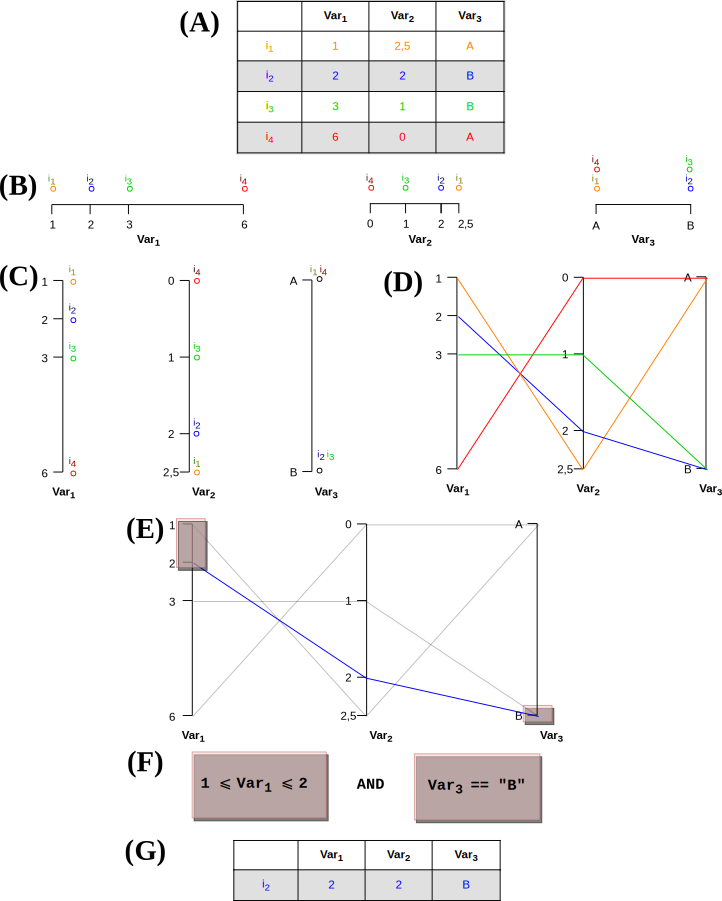
\includegraphics[width=\linewidth]{img/ParCoords_Brush.pdf}
			\caption{Démarche de construction (\textbf{A}--\textbf{D}) et de sélection par \textit{brushing} (\textbf{E}--\textbf{G}) dans un graphique en coordonnées parallèles.}
			\label{fig:schema_parcoords}
		\end{figure}

	\end{encadre}



	De plus, en matière d'interaction, on utilise fréquemment les graphiques en coordonnées parallèles en vue de filtrage, le plus souvent par des actions de \textit{brushing} (\og brossage\fg{}, c'est-à-dire sélection graphique d'une zone en dessinant son étendue à la souris -- cf. \cref{enc:parcoords}).
	Ce type de sélection se révèle en effet souvent plus efficace et intuitive qu'une sélection textuelle plus systématique :

	\begin{quotation}
		\og Filtering is an operation that removes signals from its input. A filter reduces the number of lines to be rendered. In 	this sense, dynamic querying [...] is a filter, if implemented with brushing [...], which reduces clutter by putting the filtered lines in focus using some highlighting mechanism. Combining simple brushes using logical operators [...] further allows the user to formulate rather complex queries that might even achieve faster and more accurate results using parallel coordinates than using a Structured Query Language (SQL) [...].\fg{}\\
		\mbox{}~ \hfill \cite[p. 13]{heinrich_state_2013}
	\end{quotation}

	Appliqué aux données de SimFeodal, cette interface (\cref{fig:simvadb_dashboard}) se révèle particulièrement efficace pour sélectionner les configurations de paramètres à explorer.
	Ainsi, en \og brossant \fg{} quelques filtres manuellement (\cref{fig:simvadb_dashboard} - \textbf{A}), on arrive rapidement à isoler une expérience spécifique.

	\begin{figure}[H]
		\captionsetup{width=\linewidth}
		\includegraphics[width=\linewidth]{img/SimVADB_Dashboard2.png}
		\caption{SimVADB (Simulation Visual Analysis DashBoard), un \textit{dashboard} d'exploration visuelle des indicateurs de sortie de simulation de SimFeodal.\\
		La selection des simulations à explorer se fait dans le graphique en coordonnées parallèles (\textbf{A}), en \og brossant\fg{} des filtres graphiques sur les \og dimensions\fg{} du graphique, dimensions dont les intitulés sont explicités dans le tableau (\textbf{B}).
		Les graphiques \hl{\textbf{C}} et \hl{\textbf{D}} indiquent l'évolution des types de déplacements des foyers paysans au cours des simulations.\\
		- Le graphique \hl{\textbf{C}} représente, pour cet indicateur, une moyenne de l'ensemble des simulations intégrées dans la base de données (260 ici), recouvrant donc plusieurs valeurs de paramètres.\\
		- Le graphique \hl{\textbf{D}} représente cet indicateur calculé depuis un sous-ensemble de 20 simulations (donc une expérience composée de 20 réplications), pour lesquelles le paramètre \og \texttt{X} \fg{}(\hl{Retrouver nom de ce paramètre}) vaut \texttt{true}.}
		\label{fig:simvadb_dashboard}
	\end{figure}

	Afin de permettre aux utilisateurs de remarquer les particularités des simulations explorées, nous avons choisi de mettre en emphase les différences entre la tendance générale des indicateurs, en calculant des moyennes de l'ensemble des simulations (\cref{fig:simvadb_dashboard} - \textbf{C}), et les valeurs spécifiques des indicateurs de l'expérience choisie (\cref{fig:simvadb_dashboard} - \textbf{D}).
	Cela permet, visuellement, d'être en mesure d'évaluer les sorties de simulation d'une expérience tout en ayant un référentiel visible.
	Les différentes expériences produisent des résultats sensiblement similaires\footnote{
		Si chaque expérience, et chaque réplication, produisent des résultats uniques, le choix d'une évaluation par des indicateurs visuels peut prêter à confusion si l'on n'a pas de repère précis.
		Les critères attendus, présentés dans \hl{le chapitre 3} sont ainsi assez précis pour départager une simulation très éloignée des attentes et une autre simulation plus conforme.
		Pour autant, par exemple quand les valeurs de paramètres varient faiblement, les résultats produits peuvent être assez similaires dans les grandes tendances qu'ils font ressortir.

	}, et on ne peut alors plus les comprendre sans les confronter à d'autres résultats similaires.
	Le choix d'une agrégation de l'ensemble des simulations effectuées est discutable, en ce qu'on aurait par exemple pu plutôt isoler des simulations \og de référence \fg{} afin de diminuer l'effet \og d’aplatissement \fg{} engendré par l'agrégation de résultats nombreux et hétérogènes.
	Toutefois, la variabilité des résultats étant encore assez restreinte, au moment de la création et de l'utilisation de SimVADB, ce référentiel agrégé permettait déjà une compréhension plus fine des sorties de simulations, en particulier dans l'analyse de l'impact de variations fines de valeurs de paramètres.

	\subsection{Explorer en comparant : SimEDB}

	Après le travail de paramétrage grossier qui a permis de stabiliser les mécanismes, le paramétrage de SimFeodal est entré dans une phase plus fine, visant à mieux calibrer le modèle à l'aide de variations de valeurs de paramètres de granularités inférieures.

	Dans ce cadre, par exemple en faisant varier le nombre de foyers paysans de $4000$ à $4200$ ($5\%$ de variation), les résultats du modèle changent peu :  de faibles variations de valeurs de paramètres entraînent le plus souvent de faibles variations dans les indicateurs de sorties observés\footnote{
	On peut de plus noter que, les variations n'étant pas linéaires, les répercussions d'un changement de valeur de paramètre peuvent être très différentes de l'ordre de grandeur de ce changement de valeur. Par exemple, pour ces $5\%$ de variation dans le nombre de foyers paysans, la majorité des indicateurs variera de moins de $1\%$.
	}.

	En vue d'évaluer les simulations, et donc de les différencier les unes des autres à l'aune des indicateurs générés, la comparaison d'une expérience spécifique avec un référentiel constitué de toutes les expériences précédentes ne permet plus de mener ce travail de comparaison fine : par rapport à une référentiel unique, soit-il constitué d'une agrégation de simulations ou même d'une version \og de base\fg{} du modèle (par exemple les versions principales identifiées dans le \hl{chapitre 4}), les variations sont trop fines pour être distinguables les unes des autres.

	Pour pouvoir correctement évaluer les apports d'un nouveau jeu de valeurs de paramètres, et donc, dans une démarche itérative, pouvoir différencier deux expériences successives, il est donc nécessaire d'être en mesure de comparer directement les expériences les unes avec les autres.
	Il est donc indispensable de ne plus mener une comparaison visuelle entre un référentiel commun et une expérience spécifique, mais bien de baser l'évaluation sur la comparaison entre cette expérience spécifique et une autre expérience, tout aussi spécifique.

	D'un point de vue méthodologique, cela requiert de pouvoir afficher conjointement les indicateurs de sorties de deux expériences isolées de la masse des simulations.

	La sélection d'une expérience via l'usage de \textit{brushing} sur un graphique en coordonnées parallèles des valeurs de paramètres ayant montré son efficacité, il a été choisi d'étendre ce principe d'interactivité au choix du référentiel, c'est-à-dire de baser l'évaluation non plus sur la sélection d'une expérience spécifique, mais de deux expériences spécifiques.

	\clearpage
	\begin{figure}[H]
		\centering
		\includegraphics[width=.94\linewidth]{img/SimEDB_nombreFP_villages_rotate.png}
		\caption{SimEDB }
		\label{fig:simedb_villages}
	\end{figure}
\clearpage

	Dans cette version remaniée de la plate-forme d'exploration, renommée pour l'occasion SimEDB (\textbf{Sim}Feodal \textbf{E}xploration \textbf{D}ash\textbf{B}oard)\footnote{
		La plate-forme d'exploration SimVADB (SimFeodal Visual Analysis Dashboard) a été renommée SimEDB ([...] Exploration Dashboard) par soucis de simplicité, le terme \og Exploration\fg{} nous semblant plus compréhensible et explicite que celui de Visual Analysis. Cela permet de plus une cohérence sémantique entre plusieurs productions de l'auteur -- TimeLineEDB - \autocite{cura_timelineedb_2017}; RoadTrafficEDB et CitiBikeEDB - \autocite{cura_making_2017} --, inscrivant cette plate-forme d'exploration de données issues de simulation dans une \og famille \fg{} d'outils d'exploration de données spatio-temporelles.
	}, l'accent est donc mis sur la comparaison de deux ensembles de résultats, chacun répondant à une sélection propre.
	En superposant les graphiques et tableaux des indicateurs, la comparaison visuelle est facilitée.
	On peut alors aussi bien comparer deux variations fines d'un mécanisme -- en sélectionnant par exemple une unique différence dans les valeurs de paramètres (par exemple le nombre de foyers paysans présents à l'initialisation du modèle dans les villages (\cref{fig:simedb_villages}))) --, ou encore comparer les différences entre une version stable et les expériences en découlant -- en sélectionnant, par exemple dans la partie supérieure, une version que l'on estime suffisamment aboutie pour constituer un référentiel, et dans la partie inférieure, une série d'expériences issues de ce référentiel et qui font varier plusieurs paramètres.


	\paragraph*{}
	Nous reviendrons plus précisément et longuement sur la description de SimEDB dans les parties suivantes (\cref{sec:SimEDB}, p. \pageref{sec:SimEDB}), mais après en avoir décrit les étapes de construction et les besoins auxquelles ces évolutions répondaient, il est maintenant nécessaire de revenir sur les données manipulées par cette plate-forme d'exploration.
	Le type, la structure et la masse de ces données (\cref{sec:sorties-simfeodal}) sont en effet indissociables des choix méthodologiques effectués pour SimEDB.
	Il est donc important de présenter les choix et contraintes de ces données avant d'entrer dans une description approfondie de la plate-forme.

\section{Organiser les données}
	\subsection{Modèle de données}
	\subsection{Assurer la capacité d'interrogation des données}
		\subsubsection{Interroger de manière universelle}
		\subsubsection{Interroger rapidement}
	\subsection{Assurer la pérennité et la stabilité des données}
		\subsubsection{Stockage fichier vs BDD vs projet de recherche}
	\subsection{Présentation de la/des solution(s) adoptée(s)}
		\subsubsection{Historique et raisons}
		\subsubsection{MapD}
	
\section{Une plate-forme d'exploration de données de simulations : SimEDB}
	\subsection{Contraintes}
		\subsubsection{Efficacité}
		\subsubsection{Interopérabilité}
		\subsubsection{Adaptabilité}
		\subsubsection{Généricité / indépendance aux données}

	\subsection{SimVADB / SimEDB}
		\subsubsection{Choix des technologies}
		\subsubsection{Choix de l'organisation}
		\subsubsection{Choix des modes d'interactions}
		\subsubsection{Présentation générale}

% Pour compilation finale, décommenter la dernière ligne :
% Permet d'enlever la page vide après le chapitre, mais bloque la création du minitoc. A faire donc après avoir recompilé une dernière fois avec le minitoc
%\let\clearpage\relax
% -> Remplacé pas l'usage de newclude::include*{}
